% 请确保文件编码为utf-8,使用XeLaTex进行编译,或者通过overleaf进行编译

\documentclass[answers]{exam}  % 使用此行带有作答模块
% \documentclass{exam} % 使用此行只显示题目

\usepackage{xeCJK}
\usepackage{zhnumber}
\usepackage{graphicx}
\usepackage{hyperref}
\usepackage{amsmath}
\usepackage{booktabs}
\usepackage{enumerate}
\usepackage{amssymb}
\usepackage{listings}
\usepackage{floatrow}
\usepackage{blindtext}
\usepackage{subcaption}
\pagestyle{headandfoot}
\firstpageheadrule
\firstpageheader{南京大学}{机器学习导论}{习题三}
\runningheader{南京大学}
{机器学习导论}
{习题二}
\runningheadrule
\firstpagefooter{}{第\thepage\ 页(共\numpages 页)}{}
\runningfooter{}{第\thepage\ 页(共\numpages 页)}{}


\setlength\linefillheight{.5in}

\renewcommand{\solutiontitle}{\noindent\textbf{解:}\par\noindent}

\renewcommand{\thequestion}{\zhnum{question}}
\renewcommand{\questionlabel}{\thequestion .}
\renewcommand{\thepartno}{\arabic{partno}}
\renewcommand{\partlabel}{\thepartno .}

\lstset{language=Matlab}%这条命令可以让LaTeX排版时将Matlab关键字突出显示
\lstset{
	breaklines,%这条命令可以让LaTeX自动将长的代码行换行排版
	basicstyle=\footnotesize\ttfamily, % Standardschrift
	backgroundcolor=\color[rgb]{0.95,0.95,0.95},
	keywordstyle=\color{blue},
	commentstyle=\color{cyan},
	tabsize=4,numbers=left,
	numberstyle=\tiny,
	frame=single,
	%numbers=left, % Ort der Zeilennummern
	numberstyle=\tiny, % Stil der Zeilennummern
	%stepnumber=2, % Abstand zwischen den Zeilennummern
	numbersep=5pt, % Abstand der Nummern zum Text
	tabsize=2, % Groesse von Tabs
	extendedchars=false, %
	breaklines=true, % Zeilen werden Umgebrochen
	keywordstyle=\color{red},%这一条命令可以解决代码跨页时, 章节标题, 页眉等汉字不显示的问题
	stringstyle=\color{white}\ttfamily, % Farbe der String
	showspaces=false, % Leerzeichen anzeigen ?
	showtabs=false, % Tabs anzeigen ?
	xleftmargin=17pt,
	framexleftmargin=17pt,
	framexrightmargin=5pt,
	framexbottommargin=4pt,
	%backgroundcolor=\color{lightgray},
	showstringspaces=false % Leerzeichen in Strings anzeigen ?
}
\renewcommand{\lstlistingname}{CODE}
\lstloadlanguages{% Check Dokumentation for further languages ...
	%[Visual]Basic
	%Pascal
	%C
	Python
	%XML
	%HTML
	%Java
}
%%% load AMS-Latex Package
\usepackage{amssymb}
\usepackage{amsmath,amsfonts}
% \usepackage{amsthm}
\usepackage{amsopn}
\usepackage{bm} % bold symbol
\usepackage{multirow}



% operator in optimization
\DeclareMathOperator{\argmax}{arg\,max}
\DeclareMathOperator{\argmin}{arg\,min}
\DeclareMathOperator{\softmax}{softmax}

% special functions
\newcommand{\trace}[1]{\operatornamewithlimits{tr}\left\{#1\right\}}
\newcommand{\diag}{\operatornamewithlimits{diag}}
\newcommand{\sign}{\operatornamewithlimits{sign}}
\newcommand{\const}{\operatornamewithlimits{const}}

% special display
\newcommand{\parde}[2]{\frac{\partial #1}{\partial  #2}}

% define vector and matrix symbols
\newcommand{\vct}[1]{\boldsymbol{#1}} % vector
\newcommand{\mat}[1]{\boldsymbol{#1}} % matrix
\newcommand{\cst}[1]{\mathsf{#1}}  % constant

% shorthand
\newcommand{\vtheta}{\vct{\theta}}
\newcommand{\vmu}{\vct{\mu}}
\newcommand{\vc}{\vct{c}}
\newcommand{\vp}{\vct{p}}
\newcommand{\vq}{\vct{q}}
\newcommand{\vx}{{\vct{x}}}
\newcommand{\vy}{\vct{y}}
\newcommand{\vz}{{\vct{z}}}
\newcommand{\vu}{\vct{u}}
\newcommand{\vo}{{\vct{o}}}
\newcommand{\va}{\vct{a}}
\newcommand{\vb}{\vct{b}}
\newcommand{\ve}{\vct{e}}
\newcommand{\vr}{\vct{r}}
\newcommand{\vt}{\vct{t}}
%\newcommand{\vpsi}{\vct{\psi}}
\newcommand{\vs}{\vct{s}}
\newcommand{\vv}{\vct{v}}
\newcommand{\vw}{\vct{w}}
\newcommand{\vzero}{\vct{0}}
\newcommand{\vf}{\vct{f}}
\newcommand{\vh}{\vct{h}}
\newcommand{\vg}{\vct{g}}
\newcommand{\vphi}{\vct{\phi}}
\newcommand{\vpsi}{\vct{\psi}}
\newcommand{\ones}{\vct{1}}
\newcommand{\mU}{\mat{U}}
\newcommand{\mA}{\mat{A}}
\newcommand{\mB}{\mat{B}}
\newcommand{\mC}{\mat{C}}
\newcommand{\mD}{\mat{D}}
\newcommand{\mV}{\mat{V}}
\newcommand{\mW}{\mat{W}}
\newcommand{\mH}{\mat{H}}
\newcommand{\mI}{\mat{I}}
\newcommand{\mP}{\mat{P}}
\newcommand{\mS}{\mat{S}}
\newcommand{\mJ}{\mat{J}}
\newcommand{\mM}{\mat{M}}
\newcommand{\mT}{\mat{T}}
\newcommand{\mZ}{\mat{Z}}
\newcommand{\mO}{\mat{O}}
\newcommand{\mX}{\mat{X}}
\newcommand{\mY}{\mat{Y}}
\newcommand{\mQ}{\mat{Q}}
\newcommand{\mLambda}{\mat{\Lambda}}
% \newcommand{\mL}{\mat{L}}
\newcommand{\mmI}{\mat{I}}
\newcommand{\mK}{\mat{K}}
\newcommand{\mSigma}{\mat{\Sigma}}
\newcommand{\mOmega}{\mat{\Omega}}
\newcommand{\cC}{\cst{C}}
\newcommand{\cM}{\cst{M}}
\newcommand{\cN}{\cst{N}}
\newcommand{\cQ}{\cst{Q}}
\newcommand{\cD}{\cst{D}}
\newcommand{\cL}{\cst{L}}
\newcommand{\cK}{\cst{K}}
\newcommand{\cH}{\cst{H}}
\newcommand{\cR}{\cst{R}}
\newcommand{\cU}{\cst{U}}
\newcommand{\cS}{\cst{S}}
\newcommand{\cX}{\cst{X}}
\newcommand{\sQ}{\mathcal{Q}}
\newcommand{\sS}{\mathcal{S}}
\newcommand{\sF}{\mathcal{F}}
\newcommand{\sC}{\mathcal{C}}
\newcommand{\sX}{\mathcal{X}}
\newcommand{\sH}{\mathcal{H}}

\newcommand{\bE}{\mathbb{E}}
\newcommand{\bR}{\mathbb{R}}
\newcommand{\bH}{\mathbb{H}}

\usepackage{algorithm}  
% \usepackage{algorithmic}
%\usepackage{algorithmicx}  
\usepackage{algpseudocode}  

\floatname{algorithm}{算法}  
\renewcommand{\algorithmicrequire}{\textbf{输入:}}  
\renewcommand{\algorithmicensure}{\textbf{输出:}}  

\begin{document}
\Large
\noindent 
% 姓名学号
姓名:杜兴豪 \\
学号:201300096 \\
\begin{questions}
\question [20] \textbf{利用信息熵进行决策树划分}

\begin{enumerate}
    \item  对于不含冲突样本(即属性值相同但标记不同的样本)的训练集, 必存在与训练集一致(训练误差为0)的决策树. 如果训练集可以包含无穷多个样本, 是否一定存在与训练集一致的深度有限的决策树? 并说明理由 (仅考虑每次划分仅包含一次属性判断的决策树).
    \item 
    信息熵$\operatorname{Ent}(D)$定义如下
    \begin{align}
        \operatorname{Ent}(D)=-\sum_{k=1}^{|\mathcal{Y}|}\; p_{k} \log_{2} p_{k}\label{ch4_eq:entropy}
    \end{align}
    请证明信息熵的上下界为
     \begin{equation}
        0 \leq \operatorname{Ent}(D)\leq \log _{2}|\mathcal{Y}|
    \end{equation}
    并给出等号成立的条件. 
	\item  在ID3决策树的生成过程中, 需要计算信息增益(information gain)以生成新的结点. 设离散属性$a$有$V$个可能取值$\left\{a^{1}, a^{2}, \cdots, a^{V}\right\}$, 请考教材4.2.1节相关符号的定义证明:
    \begin{equation}
        \operatorname{Gain}(D, a)=\operatorname{Ent}(D)-\sum_{v=1}^{V} \frac{\left|D^{v}\right|}{|D|} \operatorname{Ent}\left(D^{v}\right) \geq 0
    \end{equation}
    即信息增益非负.
\end{enumerate}
	\begin{solution}
		1.\\
        一定存在。由于样本中属性个数为有限个,记属性个数为$d$。若不包含冲突样本,则这些属性的任意组合最多只有$\prod_{d}m_i$种,其中$m_i$为每种属性的取值数目。则无穷多个样本中剩下的均为重复样本,可以忽略,下证该决策树为有限的。\\
        由题干信息可知道,对于不含冲突样本的训练集,一定存在一棵和训练集一致的决策树。考虑最坏情况,对每种样本都独立判断(有一个独立的叶子节点),一共仅$\prod_dm_i$个叶子节点,因此树为有限的。\\
        2.\\
        由信息熵的定义有:
        $$\begin{aligned}
            \operatorname{Ent}(D)&=-\sum_{k=1}^{|\mathcal Y |}\; p_{k}\log_{2}p_{k}=-\sum_{k=1}^{|\mathcal Y |}\;\log_2{p_{k}}^{p_k}=-\log_2\prod_{k=1}^{|\mathcal Y|}{p_k}^{p_k}
        \end{aligned}$$
        因为$0\le p_k\le 1$,我们令:
        $$f(x)=x^x=e^{x\ln x},0\le x\le 1$$
        讨论$f(x)$取值情况如下:
        $$f'(x)=\frac{\partial f(x)}{\partial x}=x^x(\ln x + 1)$$
        由$f(x)=e^{x\ln x}>0$,知
        $$
            \left\{\begin{aligned}
                &f'(x)<0&&0<x<e^{-1}\\
                &f'(x)>0&&x>e^{-1}\\
            \end{aligned}\right.
        $$
        因此
        $$
                \max f(x)=\max\{f(0), f(1)\}= 1
        $$
        我们有:
        $$\operatornamewithlimits{Ent}(D)\ge -\log_2\prod^{|\mathcal Y|}_{k=1}1=0$$
        又$p_k$为第$k$类样本在总体$D$中所占的比例,因此有:
        $$\sum^{|\mathcal Y|}_{k=1}p_k=1$$
        故取等号时,$p_k=|\mathcal Y|=1$,即一共仅一类时取等号,下证:
        $$\operatornamewithlimits{Ent}(D)\le\log_2|\mathcal Y|$$
        即解凸优化问题:
        $$\begin{aligned}
            &\max -\log_2\prod_{k=1}^{|\mathcal Y|}{p_k}^{p_k}\\
            &\mathbf{\ s.t.}\sum^{|\mathcal Y|}_{k=1}p_k=1\\
        \end{aligned}$$
        构造$\mathbf{Lagrange}$对偶问题:
        $$\max\ L(p_1,\dots,p_{|\mathcal Y|},\lambda)=-\log_2\prod_{k=1}^{|\mathcal Y|}{p_k}^{p_k}+\lambda\left(\sum^{|\mathcal Y|}_{k=1}p_k-1 \right)$$
        分别求偏导有:
        $$\begin{aligned}
            &\frac{\partial L(p_1,\dots,p_{|\mathcal Y|},\lambda)}{\partial p_k}=-\log_2p_k-1+\lambda\\
            &\frac{\partial L(p_1,\dots,p_{|\mathcal Y|},\lambda)}{\partial \lambda}=\sum^{|\mathcal Y|}_{k=1}p_k-1\\
        \end{aligned}$$
        令上式全为0,有:
        $$\begin{aligned} 
            &p_k=2^{\lambda-1}\\
            &\sum^{|\mathcal Y|}_{k=1}p_k=|\mathcal Y|2^{\lambda-1}=1\\
        \end{aligned}$$
        得到对偶问题的解(同时也是原优化问题的解)为:
        $$p_1=p_2=\cdots=p_{|\mathcal Y|}=\frac1{|\mathcal Y|}$$
        此时得到信息熵的最大值:
        $$
        \max \operatornamewithlimits{Ent}(D)=-\sum^{|\mathcal Y|}_{k=1}\frac1{|\mathcal Y|}\log_2{\frac1{|\mathcal Y|}}=\log_2{|\mathcal Y|}
        $$
        即
        $$
        \operatornamewithlimits{Ent}(D)\le\log_2{|\mathcal Y|}
        $$
        由优化问题同样可以知道取等条件为:
        $$p_1=p_2=\cdots=p_{|\mathcal Y|}=\frac1{|\mathcal Y|}$$
        3.\\
        假设全集$D$中,第$k$类样本的元素个数为$m_k$,则在$D^v$中第$k$类样本所占比例为:
        $$p_k^v=\frac{m_k}{|D^v|}$$
        则其信息熵可以表示为:
        $$\operatornamewithlimits{Ent}(D^v)=-\sum^{|\mathcal Y|}_{k=1}\frac{m_k}{|D^v|}\log_2{\frac{m_k}{|D^v|}} $$\\
        则有
        $$\sum^V_{v=1}\frac{|D^v|}{|D|}\operatornamewithlimits{Ent}(D^v)=-\sum^V_{v=1}\sum^{|\mathcal Y|}_{k=1}\frac{m_k}{|D|}\log_2{\frac{m_k}{|D^v|}} $$\\
        而
        $$\operatorname{Ent}(D)=-\sum_{k=1}^{|\mathcal{Y}|}\; p_{k} \log_{2} p_{k}=-\sum^V_{v=1}\sum^{|\mathcal Y|}_{k=1}\frac{m_k}{|D|}\log_2\frac{m_k}{|D|} $$
        即证明
        $$\begin{aligned}
            &-\log_2{\frac{m_k}{|D^v|}}\le -\log_2{\frac{m_k}{|D|}}\\
            &\iff \frac1{|D^v|}\ge \frac1{|D|}\\
        \end{aligned}$$
        由于$|D^v|$为包含D中所有在属性$a$上取值为$a^v$的样本,因此一定有
        $$|D|\ge |D^v|$$
        上式成立,证明完毕。
    \end{solution}


\question [15] \textbf{决策树划分计算} \label{ch4_prob:get_tree}

本题主要展现决策树在不同划分标准下划分的具体计算过程. 假设一个包含三个布尔属性$X, Y, Z$的属性空间, 目标函数$f=f(X, Y, Z)$作为标记空间, 它们形成的数据集如\ref{ch4_tab:bool_table}所示. 
\begin{table}[ht]
    \centering
    \caption{布尔运算样例表}\label{ch4_tab:bool_table}
    \tabcolsep 15pt
    \begin{tabular}{cccc|c||cccc|c}
        \hline 
        编号 & $X$ & $Y$ & $Z$ & $f$ & 编号 & $X$ & $Y$ & $Z$ & $f$ \\
        \hline 1 & 1 & 0 & 1 & 1 & 5 & 0 & 1 & 0 & 0\\
        2 & 1 & 1 & 0 & 0 & 6 & 0 & 0 & 1 & 0 \\
        3 & 0 & 0 & 0 & 0 & 7 & 1 & 0 & 0 & 0\\
        4 & 0 & 1 & 1 & 1 & 8 & 1 & 1 & 1 & 0\\
        \hline
    \end{tabular}
\end{table}
\begin{enumerate}
    \item 请使用信息增益作为划分准则画出决策树的生成过程. 当两个属性信息增益相同时, 依据字母顺序选择属性. 
    \item 请使用基尼指数作为划分准则画出决策树的生成过程, 当两个属性基尼指数相同时, 依据字母顺序选择属性. 
\end{enumerate}
	
	\begin{solution}
		1.\\
        令全集为D,$|D|=8$,其中正例有2个,反例6个,则当前根节点的信息熵为:
        $$\operatornamewithlimits{Ent}(D)= -\left(\frac14\log_2{\frac14}+\frac34\log_2{\frac34} \right)=0.8113$$
        以X属性划分,有两个取值,其中当$X=1$时有4个样例,正例1个,反例3个;当$X=0$时共4个样例,正例1个,计算信息熵为:
        $$\begin{aligned}
            &\operatornamewithlimits{Ent}(D^{X_1}) = -\left(\frac14\log_2{\frac14}+\frac34 \log_2{\frac34} \right)=0.8113\\
            &\operatornamewithlimits{Ent}(D^{X_0}) = -\left(\frac14\log_2{\frac14}+\frac34 \log_2{\frac34} \right)=0.8113\\
        \end{aligned}$$
        因此可计算属性X的信息增益为:
        $$\begin{aligned}
        \operatornamewithlimits{Gain}(D,X)
            &=\operatornamewithlimits{Ent}(D)-\sum^1_{v=0}\frac{|D^{X_v}|}{|D|}\operatornamewithlimits{Ent}(D^{X_v})\\
            &=0.8113-(\frac12\times0.8113+\frac12\times0.8113)\\
            &=0\\
        \end{aligned}$$
        类似可计算属性Y,Z的信息增益为:
        $$\begin{aligned}
            &\operatornamewithlimits{Gain}(D,Y)=0 \\
            &\operatornamewithlimits{Gain}(D,Z)=0.3113\\
        \end{aligned}$$
        属性Z的信息增益最大,则选用Z对根节点进行划分,得到划分情况如图所示:\\
        \centerline{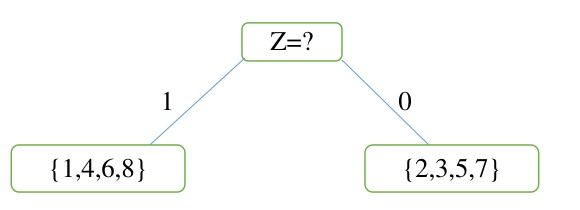
\includegraphics[width=0.7\linewidth]{Z.jpg}}\\
        其中各分支的信息熵为:
        $$
        \begin{aligned}
            &\operatornamewithlimits{Ent}(D^{Z_1})=-\left(\frac12\log_2{\frac12}+ \frac12\log_2{\frac12}\right)=1\\
            &\operatornamewithlimits{Ent}(D^{Z_0})=-\left(0+\log_2{1}\right)=0\\
        \end{aligned}
        $$
        在$Z=1$分支下,计算X,Y的信息增益如下:
        $$
        \begin{aligned}
            &\operatornamewithlimits{Gain}(D^{Z_1},X)=1\\
            &\operatornamewithlimits{Gain}(D^{Z_1},Y)=1\\
        \end{aligned}
        $$
        信息增益相同,以字典序选取X作为当前划分属性对$Z=1$分支进行划分。\\
        在$Z=0$分支下,观察到所有样例取值f均为0,因此不再继续划分。\\
        最后在X分支下以Y划分,得到最终结果如下:\\
        \centerline{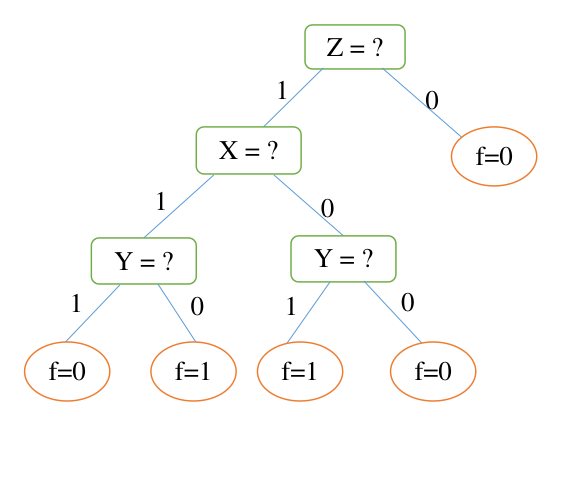
\includegraphics[width=0.7\linewidth]{ALL.png}}
        2.\\
        $$\operatornamewithlimits{Gini}(D)=1-\sum^{|\mathcal Y|}_{k=1}p_k^2=1-\left(({\frac14})^2+({\frac34})^2\right)=0.375$$\\
        以X属性划分,其取值为$X=1$和$X=0$的基尼值为:
        $$
        \begin{aligned}
            &\operatornamewithlimits{{Gini}}(D^{X_1})=1-\left(({\frac14})^2+({\frac34})^2\right)=0.375\\
            &\operatornamewithlimits{{Gini}}(D^{X_0})=1-\left(({\frac14})^2+({\frac34})^2\right)=0.375\\
        \end{aligned}
        $$
        则X属性的基尼指数为:
        $$
        \begin{aligned}
            \operatornamewithlimits{Gini\_index}(D,X)
            &=\sum^V_{v=1}\frac{|D^{X_v}|}{|D|}\operatornamewithlimits{Gini}(D^{X_v})\\
            &=\frac12\times 0.375 + \frac12\times 0.375\\
            &=0.375\\
        \end{aligned}
        $$
        类似可计算Y,Z属性的基尼指数为:
        $$
        \begin{aligned}
            &\operatornamewithlimits{Gini\_index}(D,Y)=\frac12\times0.375+\frac12\times0.375=0.375\\
            &\operatornamewithlimits{Gini\_index}(D,Z)=\frac12\times0+\frac12\times 0.5=0.25\\
        \end{aligned}
        $$
        属性Z的基尼指数最小,则选用Z对根节点进行划分,得到划分情况如图:\\
        \centerline{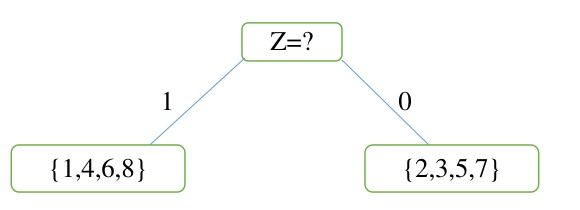
\includegraphics[width=0.7\linewidth]{Z.jpg}}\\
        其中各分支的基尼值为:\\
        $$
        \begin{aligned}
            &\operatornamewithlimits{Gini}(D^{Z_1})=0.25\\
            &\operatornamewithlimits{Gini}(D^{Z_0})=0\\
        \end{aligned}
        $$
        观察到$Z=0$时的基尼值已经为最小,是最纯净的情况,因此不用再细分。\\
        当$Z=1$时,计算X,Y的基尼指数如下:\\
        $$
        \begin{aligned}
            &\operatornamewithlimits{Gini\_index}(D^{Z_1},X)=\frac12\times0.5+\frac12\times0.5=0.5\\
            &\operatornamewithlimits{Gini\_index}(D^{Z_1},Y)=\frac12\times0.5+\frac12\times 0.5=0.5\\
        \end{aligned}
        $$
        基尼指数相同,则以字典序选取X来划分$Z=1$的情况。\\
        最后在$X$分支下以Y进行划分,得到最终结果如图:\\
        \centerline{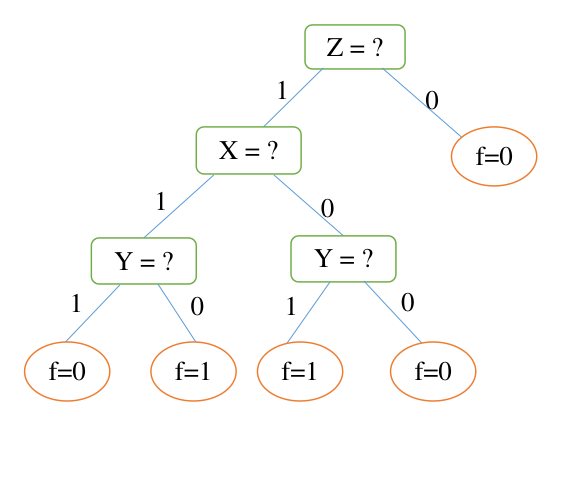
\includegraphics[width=0.7\linewidth]{ALL.png}}
    \end{solution}


\question [25] \textbf{决策树剪枝处理} \label{ch4_prob:prunning}

教材4.3节介绍了决策树剪枝相关内容, 给定包含5个样例的人造数据集如表\ref{ch4_tab:artificial_training_dataset}所示, 其中“爱运动”、“爱学习”是属性, “成绩高”是标记. 验证集如表\ref{ch4_tab:artificial_testing_dataset}所示. 使用信息增益为划分准则产生如图\ref{ch4_fig:decision_tree_1}所示的两棵决策树. 请回答以下问题: 
\begin{table}[!htb]
    \caption{人造数据集}
    \begin{minipage}[t]{.48\linewidth}
      \subcaption{训练集}\label{ch4_tab:artificial_training_dataset}
      \centering
        \begin{tabular}{cccc}
        \hline 编号 & 爱运动 & 爱学习 & 成绩高 \\
        \hline 1 & 是 & 是 & 是 \\
        2 & 否 & 是 & 是 \\
        3 & 是 & 否 & 否 \\
        4 & 是 & 否 & 否 \\
        5 & 否 & 否 & 是 \\
        \hline
\end{tabular}
    \end{minipage}%
    \begin{minipage}[t]{.48\linewidth}
      \centering
        \subcaption{验证集}\label{ch4_tab:artificial_testing_dataset}
        \begin{tabular}{cccc}
		\hline 编号 & 爱运动 & 爱学习 & 成绩高 \\
		\hline 6 & 是 & 是 & 是 \\
		7 & 否 & 是 & 否 \\
		8 & 是 & 否 & 否 \\
		9 & 否 & 否 & 否 \\
		\hline
		\end{tabular}
    \end{minipage} 
\end{table}
\begin{figure}[ht]
    \centering
    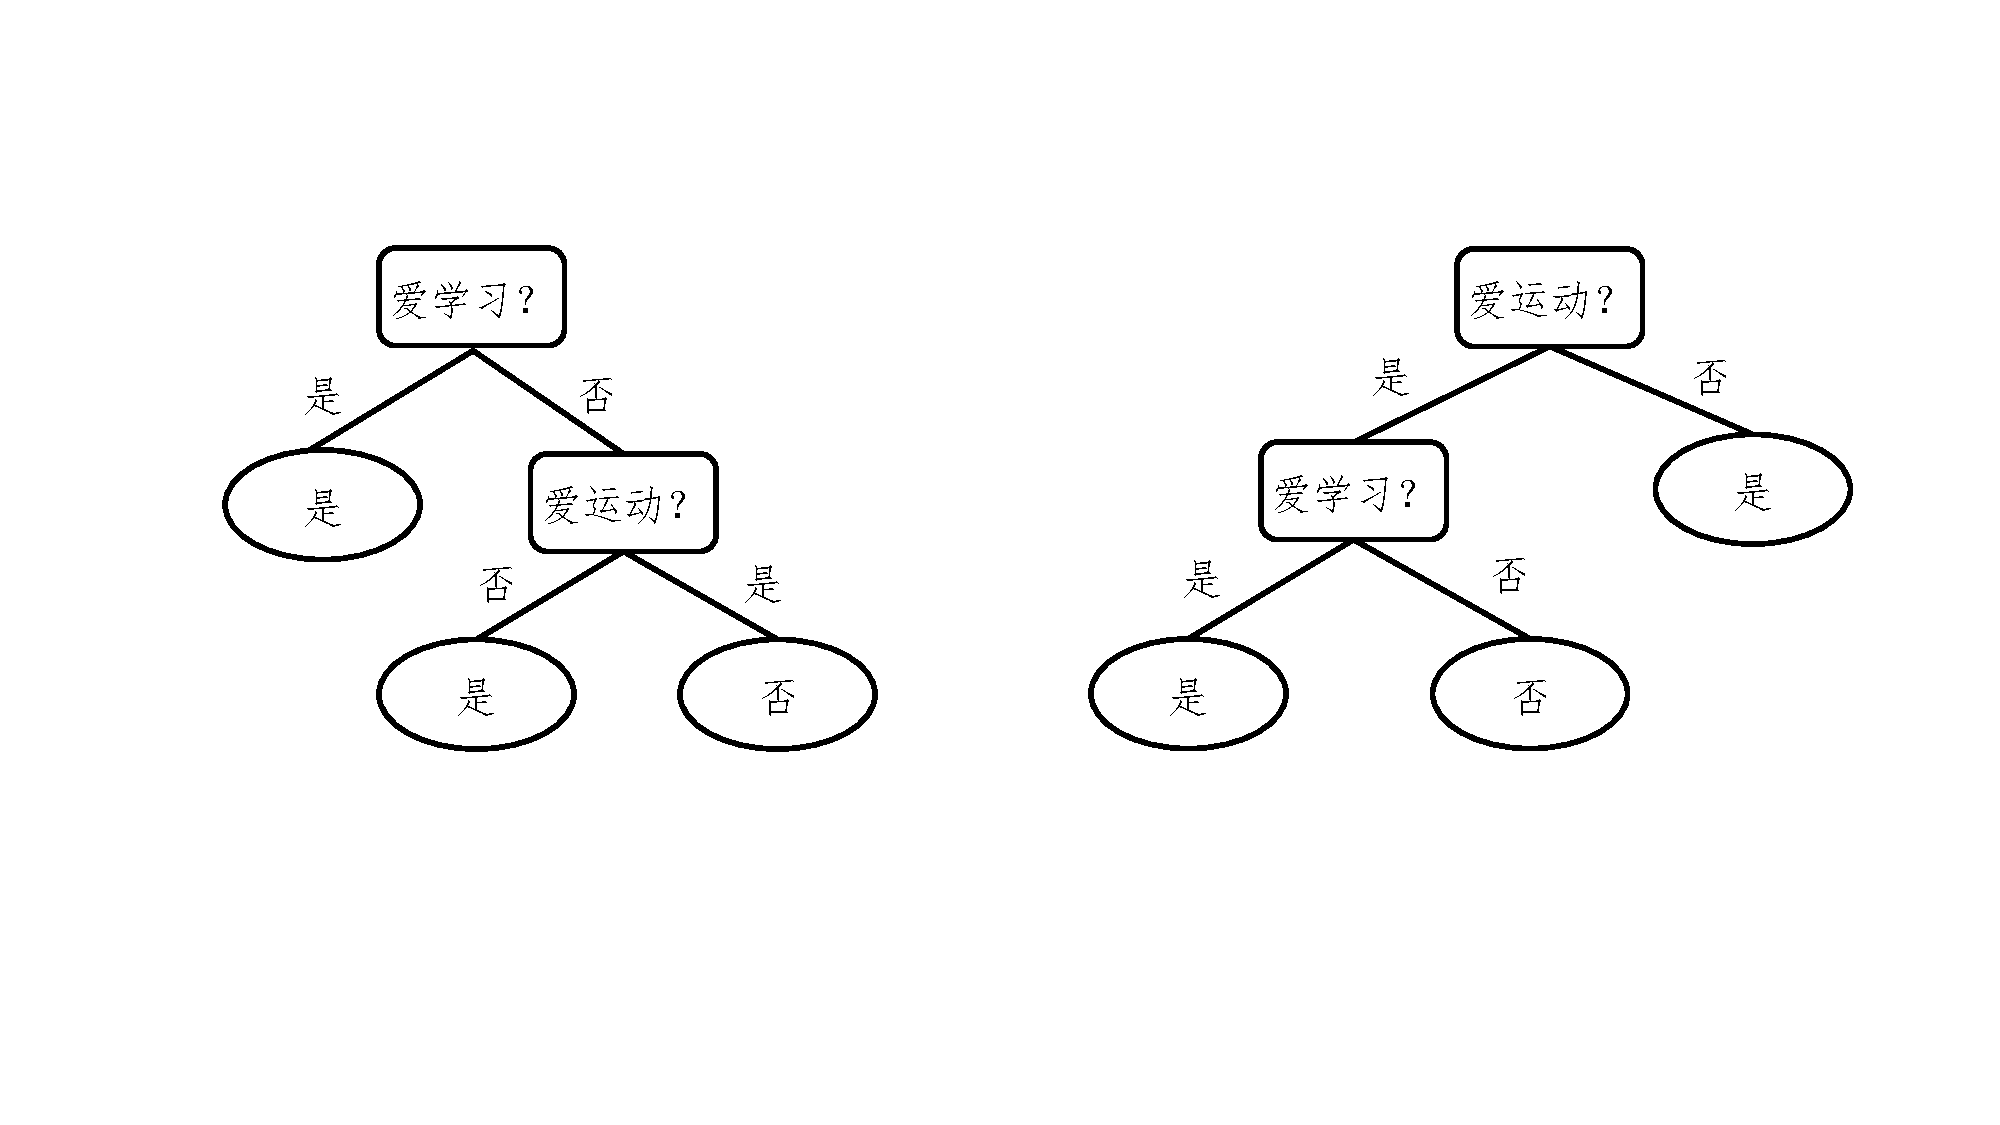
\includegraphics[width=0.8\textwidth]{figure/ch4_decision_tree_1.pdf}
    \caption{人造数据决策树结果}\label{ch4_fig:decision_tree_1}
\end{figure}
\begin{enumerate}
    \item 
    请验证这两棵决策树的产生过程.
    \item 
     对图\ref{ch4_fig:decision_tree_1}的结果基于该验证集进行预剪枝、后剪枝, 给出剪枝后的决策树. 
    \item
    比较预剪枝、后剪枝的结果, 每种剪枝方法在训练集、验证集上的准确率分别为多少?哪种方法拟合能力较强?
\end{enumerate}

	\begin{solution}
        1.\\
        令全集为D,则其信息熵可以表示为:
        $$\operatornamewithlimits{Ent}(D)=-\left(\frac35\log_2\frac35+\frac25\log_2\frac25 \right)=0.97095$$
        若选择爱学习来划分原数据集,以属性值“是”“否”得到其信息熵分别为:
        $$
        \begin{aligned}
            &\operatornamewithlimits{Ent}(D^1)=-\left(0+\log_21 \right)=0\\
            &\operatornamewithlimits{Ent}(D^2)=-\left(\frac13\log_2{\frac13}+\frac23\log_2\frac23 \right)=0.91830
        \end{aligned}
        $$
        则其信息增益为:
        $$
        \begin{aligned}
        \operatornamewithlimits{Gain}(D,\text{爱学习})
        &=\operatornamewithlimits{Ent}(D)-\frac25\operatornamewithlimits{Ent}(D^1)-\frac35\operatornamewithlimits{Ent}(D^2)\\
        &=0.41997
        \end{aligned}
        $$
        同理可以计算出选择爱运动划分数据集的信息增益为:
        $$\operatornamewithlimits{Gain}(D,\text{爱运动})=0.41997$$ 
        两者的信息增益相同,因此划分根节点采用哪个都合理。\\
        若选用爱学习来划分根节点\\
        由
        $$\operatornamewithlimits{Ent}(D^1)=0$$
        知道当爱学习为“是”的时候,样例绝对有序,因此不再继续展开。\\
        当爱学习为“否”的时候,以爱运动划分数据集,得到图一所示结果为合理。\\
        若采用爱运动来划分根节点\\
        同样能看出当爱运动为“否”的时候,样例中所有的标签均为“是”,因此不再展开。\\
        当爱运动为“是”的时候,以爱学习划分,得到图二所示结果也合理。\\
        2.\\
        预剪枝:\\
        若不以爱学习进行划分,将其标记为训练集中出现最多的“是”,在验证集的精度为25\%,\\
        而使用“爱学习”进行划分之后,“是”被判断为“是”(“是”爱学习被判断为“是”成绩好),“否”被判断为“否”,其验证集精度为75\%>25\%,因此需要使用“爱学习”划分根节点。\\
        若当爱学习为“否”的时候,不使用“爱运动”划分数据集,而将其标记为最多的“否”,则其验证集精度为75\%\\
        而使用“爱运动”进行划分之后,验证集精度为50\%<75\%,因此不需要继续以“爱运动”划分数据。\\
        最终得到预剪枝后的图像如下:\\
        \centerline{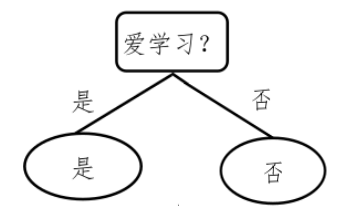
\includegraphics[width=0.5\linewidth]{prepruning.png}}\\
        后剪枝:\\
        易知完整决策树的验证集精度为50\%\\
        若将“爱运动”领衔的分支剪除,将其替换为训练集爱学习下“否”中标记最多的“否”,此时验证集精度提升为75\%>50\%,因此需要剪枝。\\
        若将“爱学习”领衔的分支剪除,将其替换为训练集中标记最多的“是”,此时验证集精度变为25\%<75\%,不剪枝。\\
        最终后剪枝图像如下:\\
        \centerline{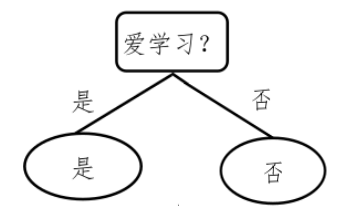
\includegraphics[width=0.5\linewidth]{prepruning.png}}\\
        3.\\
        两种方法得到的决策树完全相同,因此具有相同的准确率和拟合能力。
        训练集上准确率为80\%,测试集上准确率为75\%
	\end{solution}

\question [20] \textbf{连续与缺失值}



\begin{enumerate}
	\item 
    考虑如表~\ref{ch4_tab:continuous_small_dataset}所示数据集,仅包含一个连续属性,请给出将该属性“数字”作为划分标准时的决策树划分结果。
    \begin{table}[h]
    \begin{center}
    \begin{tabular}{cc}
    \hline 属性 & 类别 \\
    \hline 3 & 正 \\
    4 & 负 \\
    6 & 负 \\
    9 & 正 \\
    \hline
    \end{tabular}
    \caption{连续属性数据集}\label{ch4_tab:continuous_small_dataset}
    \end{center}
    \end{table}
	\item 请阐述决策树如何处理训练时存在缺失值的情况,具体如下:考虑表~\ref{ch4_tab:bool_table}的数据集,如果发生部分缺失,变成如表~\ref{ch4_tab:missing_dataset}所示数据集(假设$X, Y, Z$只有0和1两种取值).
    \begin{table}[ht]
    \centering
    \caption{缺失数据集}\label{ch4_tab:missing_dataset}
    \begin{tabular}{ccc|c}
        \hline X & Y & Z & $f$ \\
        \hline 
        1 & 0 & - & 1\\
        - & 1 & 0 & 0\\
        0 & - & 0 & 0\\
        0 & 1 & 1 & 1\\
        - & 1 & 0 & 0\\
        0 & 0 & - & 0\\
        1 & - & 0 & 0\\
        1 & 1 & 1 & 0\\
        \hline
    \end{tabular}
\end{table}
    在这种情况下,请考虑如何处理数据中的缺失值,并结合问题~\ref{ch4_prob:get_tree}第1小问的答案进行对比,论述方法的特点以及是否有局限性。
	\item 请阐述决策树如何处理测试时存在缺失值的情况,具体如下:对于问题~\ref{ch4_prob:prunning}训练出的决策树,考虑表~\ref{ch4_tab:artificial_testing_dataset2}所示的含有缺失值的测试集,输出其标签,并论述方法的特点以及是否有局限性。
	\begin{table}[ht]
    \centering
    \caption{缺失数据集}\label{ch4_tab:artificial_testing_dataset2}
	\begin{tabular}{cccc}
		\hline 编号 & 爱运动 & 爱学习 & 成绩高 \\
		\hline 6 & 是 & - &  \\
		7 & - & 是 &  \\
		8 & 否 & - &  \\
		9 & - & 否 &  \\
		\hline
	\end{tabular}
	\end{table}
    
\end{enumerate}
	\begin{solution}
	    1.\\
        \centerline{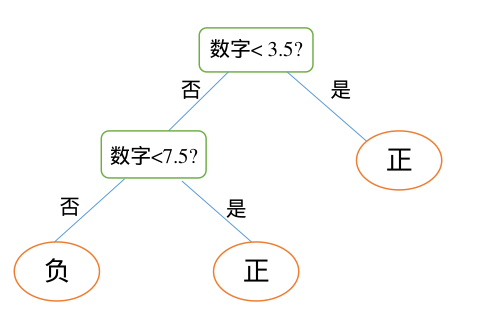
\includegraphics[width=0.5\linewidth]{4.1.png}}\\
        2.\\
        假设$\hat D$为在X属性上没有缺失的样本子集,则以这个集合为训练集计算其信息熵如下:
        $$
        \begin{aligned}
            \operatornamewithlimits{Ent}(\hat D)=-\left(\frac13\log_2\frac13+\frac23\log_2\frac23 \right)=0.91830\\
        \end{aligned}    $$
        以X属性划分,设$\hat D^1,\hat D^0$为X取值为1,0时的子集,则其信息熵:
        $$
        \begin{aligned}
            &\operatornamewithlimits{Ent}(\hat D^1)=-\left(\frac13\log_2\frac13+\frac23\log_2\frac23 \right)=0.91830\\
            &\operatornamewithlimits{Ent}(\hat D^0)=-\left(\frac13\log_2\frac13+\frac23\log_2\frac23 \right)=0.91830\\
        \end{aligned}    $$
        因此得到信息增益为:
        $$\begin{aligned}
        \operatornamewithlimits{Gain}(D,X)
            &=\frac{|\hat D|}{|D|}\operatornamewithlimits{Gain}(\hat D,X)\\
            &=\frac{|\hat D|}{|D|}\left(\operatornamewithlimits{Ent}(\hat D)-\sum^V_{v=1}\frac{|\hat D^v|}{|\hat D|}\operatornamewithlimits{Ent}(\hat D^v) \right)\\
            &=\frac34\times\left(0.91830-\left(\frac12\times0.91830+\frac12\times0.91830 \right) \right)\\
            &=0\\
        \end{aligned} $$
        同理可计算Y,Z的信息增益为:
        $$\begin{aligned}
            &\operatornamewithlimits{Gain}(D,Y)=\frac34\times\operatornamewithlimits{Gain}(\hat D,Y)=0.03308\\
            &\operatornamewithlimits{Gain}(D,Z)=\frac34\times\operatornamewithlimits{Gain}(\hat D,Z)=0.43873\\
        \end{aligned}    $$
        因此选用信息增益最大的Z进行划分。在原数据集中Z缺失的1、6号元素同时进入Z的两个分支,其权重在$Z=1$分支中为$1/3$,在$Z=0$分支中为$2/3$\\
        现在对$Z=0$分支继续划分,该分支中取值为1的权重为:
        $$p_1=\frac{\frac23}{4+2\times\frac23}=\frac18$$
        因此其信息熵为:
        $$\operatornamewithlimits{Ent}(D^{Z_0})=-\left(\frac18\log_2\frac18+\frac78\log_2\frac78 \right)=0.54356$$
        使用X属性来划分数据集$D^{Z_0}$,我们有:无缺训练集$\hat D^{Z_0}$为\{1,3,6,7\},分别计算X取值为0,1时的信息熵如下:
        $$\begin{aligned}
            &\operatornamewithlimits{Ent}(\hat D^{Z_0X_0})=-\left(0+\log_2 1 \right)=0\\
        \end{aligned} $$
        $$ \operatornamewithlimits{Ent}(\hat D^{Z_0X_1})=-\left(\frac35\log_2\frac35+\frac25\log_2\frac25 \right)= 0.97095$$
        因此可以计算出其信息增益为:
        $$
        \operatornamewithlimits{Gain}(D^{Z_0},X)=\frac{10}{16}\times\left(0.54356-\left(\frac12\times0+\frac12\times0.97095\right) \right)=0.03630
        $$
        同理可以计算出Y的信息增益为:
        $$
        \operatornamewithlimits{Gain}(D^{Z_0},Y)=\frac{10}{16}\times\left(0.54356-\left(\frac35\times0+\frac25\times  1 \right) \right)=0.08972
        $$
        因此选择信息增益较大的Y来划分$Z=0$分支。原先Y缺失的样本同时进入两个分支,在$Y=1$分支中权重为原来的$2/3$,在$Y=0$分支中为原来的$1/3$。\\
        观察到$Y=1$分支中的所有结果均为0,因此不再展开。\\
        $Y=0$分支再使用X做进一步划分,不多赘述。\\
        然后对$Z=1$分支讨论划分方法。
        $$\operatornamewithlimits{Ent}(D^{Z_1})=-\left(\frac12\log_2\frac12+\frac12\log_2\frac12 \right)=1$$
        X,Y在此样本中均无缺失,计算其信息增益分别为:
        $$\begin{aligned}
            &\operatornamewithlimits{Gain}(D^{Z_1},X)=0.18872\\
            &\operatornamewithlimits{Gain}(D^{Z_1},Y)=0\\
        \end{aligned} $$
        因此选用X划分$Z=1$分支。再使用Y划分X的分支,不多赘述。
        得到最终结果如下图:\\
        \centerline{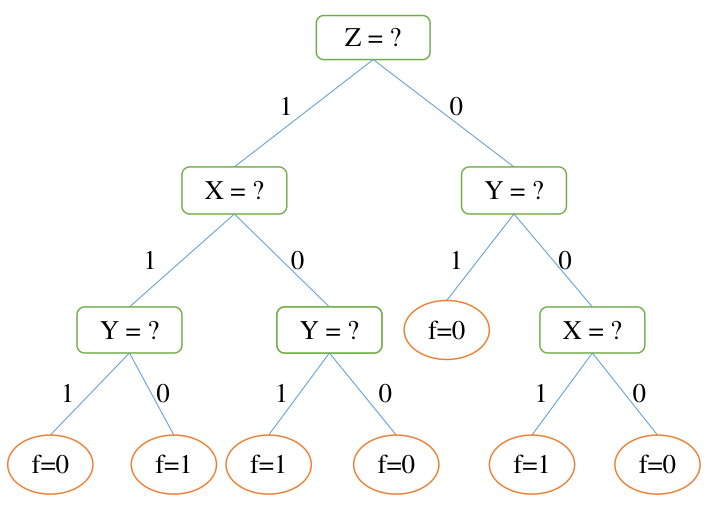
\includegraphics[width=0.9\linewidth]{4.2.png}}\\
        处理方法使用:\\
        在无缺数据集下处理数据,以频率猜测缺失样本的属性值,将有缺样本以猜测的频率分发权重,放入所有的分支中,从而可以利用好有缺样本的无缺部分。\\
        对比结果:\\
        当数据缺失时,在$Z=0$处并没有直接判断为$f=0$,而是继续用属性$Y$继续划分数据集,其余部分保持一致。\\
        特点:\\
        不用将缺失数据集丢弃,极大地提高了数据的利用率,并且学习出的决策树在大体上与无缺数据集保持一致,性能良好。\\
        对方法局限性的思考:\\
        当同一属性的样本缺失太多条时,这样的预测将变得难以保持稳定,猜测补全的结果很有可能和真实数据集发生较大的偏差。
        \\3.\\
        以频率估计概率,将原测试集缺失样本以其出现概率分发权重,创造更大的测试集,每条样本具有不同的权重。计算成功率时以加权和计算。得到的新测试集以及对应标签如下:
        \\\begin{tabular}{ccccc}
            \hline 编号 & 爱运动 & 爱学习 & 成绩高 & 权重\\
            \hline 
            6 & 是 & 是 & 是 &0.5\\
              & 是 & 否 & 否 &0.5\\
            7 & 是 & 是 & 是 &0.5\\
              & 否 & 是 & 是 &0.5\\
            8 & 否 & 是 & 是 &0.5\\
              & 否 & 否 & 否 &0.5\\
            9 & 是 & 否 & 否 &0.5\\
              & 否 & 否 & 否 &0.5\\
            \hline
        \end{tabular}\\
        特点为可以利用到缺失样本,利用率高。
        局限性是当测试集分布和真实情况很不同时,预测结果有可能发生较大偏差。
	\end{solution}


\question [20] \textbf{多变量决策树}

考虑如下包含10个样本的数据集, 每一列表示一个样本, 每个样本具有二个属性, 即$\vx_i = (x_{i1};\; x_{i2})$.
\begin{table}[ht]
    \begin{center}
    \begin{tabular}{ccccccccccc}
    \hline 编号 & 1 & 2 & 3 & 4 & 5 & 6 & 7 & 8 & 9 & 10 \\
    \hline $A_1$ & 24 & 53 & 23 & 25 & 32 & 52 & 22 & 43 & 52 & 48 \\ 
    $A_2$ & 40 & 52 & 25 & 77 & 48 & 110 & 38 & 44 & 27 & 65\\
    \hline 标记 & 1 & 0 & 0 & 1 & 1 & 1 & 1 & 0 & 0 & 1\\
    \hline
    \end{tabular}
    \end{center}
\end{table}
\begin{enumerate}
    \item 计算根结点的熵; 
    \item 构建分类决策树, 描述分类规则和分类误差; 
    \item 根据 $\alpha x_{1}+\beta x_{2}-1$,  构建多变量决策树,描述树的深度以及 $\alpha$ 和 $\beta$ 的值. 
\end{enumerate}
	\begin{solution}
	    1.\\
        令训练集为$D$,则根节点的熵为:
        $$
        \begin{aligned}
            \operatornamewithlimits{Ent}(D)
            &=-\sum^{|\mathcal Y|}_{k=1}p_k\log_2 p_k\\
            &=-\left(\frac35\log_2\frac35+\frac25\log_2\frac25 \right)\\
            &=0.97095\\
        \end{aligned}
        $$
        2.\\
        根据训练样本的图像,以及考虑的划分候选点集合
        可以得到以下分类边界:\\
        \centerline{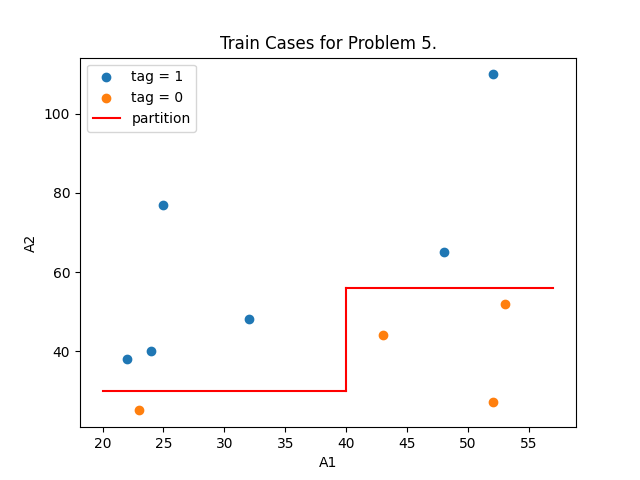
\includegraphics[width=0.82\linewidth]{5.2.png}}\\
        得到分类规则为:\\
        先以$A_2<32.5$为界,满足的为标记为0的点,否则进入分支;\\
        再以$A_1<37.5$为界限,满足的为标记为1的点,否则再进入分支;\\
        最后以$A_2< 58.5$为界限,满足的标记为0,否则标记为1。\\
        可以得到分类决策树为:\\
        \centerline{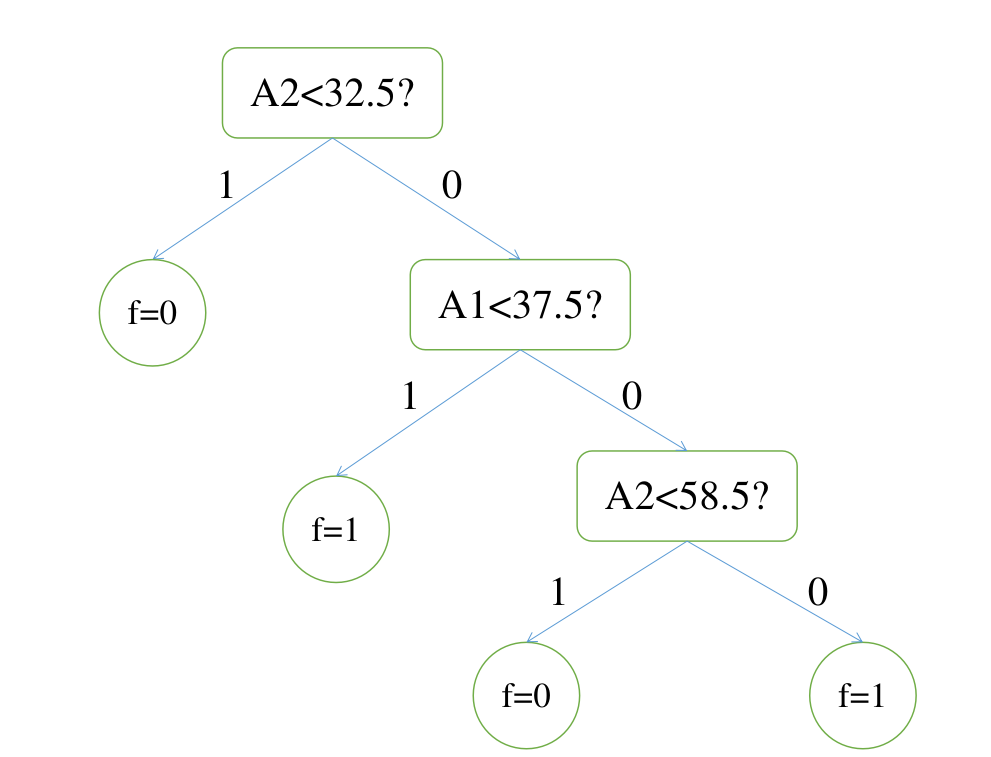
\includegraphics[width=0.82\linewidth]{5.3.png}}\\
        由图可以知道分类误差为0\%\\
        3.\\
        由图可知该分类可以通过一条直线进行划分。尝试线性分类方法。令
        $$X =
        \left(
            A_1^{\top},A_2^\top,1\right)\in\mathbb R^{10\times3}$$
        参数$\alpha,\beta$合并为
        $$ w=
        \left( 
            \begin{matrix}
             \alpha\\
             \beta \\
             b  
            \end{matrix}
        \right)\in\mathbb R^{3\times1}
        $$
        学得参数
        $$
        w^*=(X^\top X)^{-1}X^\top y=\left(
            \begin{matrix}
                -0.02264422\\
                0.01454232\\
                0.68196814
        \end{matrix} \right)
        $$
        由于题目要求为$\alpha x_1+\beta x_2-1$,因此需要在原分类器输出结果的判别条件上除以$-0.68196814$,得到如下的决策树:\\
        \centerline{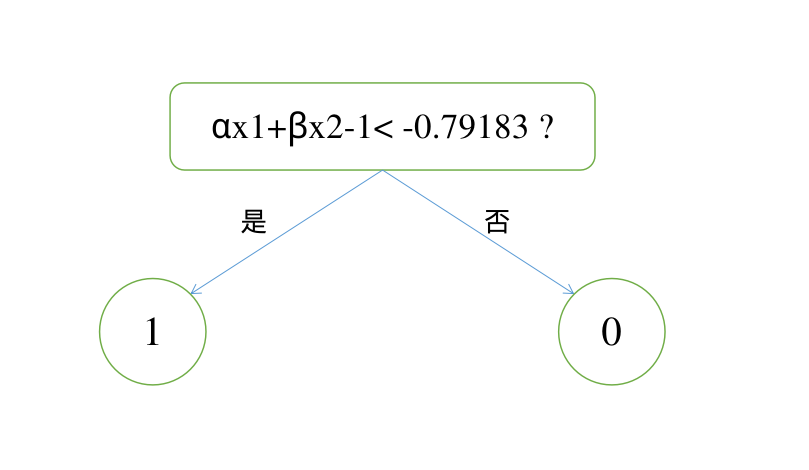
\includegraphics[width=0.82\linewidth]{5.4.png}}\\
        经验证,正确率为100\%,无需继续划分。\\
        因此树深度为2, $\alpha=0.03320422 ,\beta=-0.02132404$
	\end{solution}

\end{questions}


\end{document}